\chapter{Waypoints positioning.} 
\minitoc
To remind, the main objective is to propose a efficient path to can cover an area using a camera mounted on a UAV. The solution proposed here, is to focus on optimizing the position of a cameras set to fully cover an area in a first time. When set of optimized cameras pose is found the position can be used as waypoints for an UAVs path. Indeed find an optimized position for each camera of a given set is primordial. The following section are dedicated to the optimization of it. 




%\section{An optimization problem.}

During the previous section the problem was discussed as an optimization problem. The formulation of the problem was presented  and  the complexity of the problem was disused in the section \ref{sec:OptimizationComplexity}. Thanks to this preliminary result the folowing section is only focuse on the optimization process. 



\section{PSO.}

The PSO (Particle Swarm Optimization) is an algorithm dedicated to the optimization problems. It is an stochastic algorithms form the family of evolutionary algorithms (see \ref{chap:EA}). 
The PSO is a relatively young compared then the other EA. It was developed by Russel Eberhart and James Kennedy in 1995 [148* bis]. The concept of PSO is to optimize iteratively a continuous non linear function. To do that the PSO is inspired by the behaviour of animals. As it append here form the bird flocking, fish schooling and swarming theory. These animals working in group to find food. 
The direction to take is not decide by one leader, but by all individuals of the swarm by relaying just few informations as what quantities of food their found. 
The swarm composed by numerous individuals became smarter and more efficient to reach their objective. 
The algorithm proposed by Russel Eberhart and James Kennedy in [148* bis] are directly inspired by these behaviours.

The methodologies used is to consider each individual or also called particles as a solution of the problems. The problems is optimized at each iteration. To do that each solution must be comparable and quantifiable. At each iteration, each particle have to be tested by a cost function in order to discriminate the best particles of the swarm. The cost function and the design of it has been detailed in the section \ref{chap:formulation}.
When the best particle is found at the end of an iteration, the other particles of set try to change their initial direction to converge more or less quickly to the actual best. 
Indeed the power of this algorithm is to have a very basic individuals behaviour to guide the particles. 
Each particles are guided by 3 behaviours.
 \begin{itemize}
 \item  This own velocity $V_k$. 
 \item  This own best solution $P_i$.
 \item  The best solution $P_g$.
\end{itemize}  
Here the velocity represent the useful speed of the particle to converge to the best solution. More the velocity is high more the step at each iteration will be long. 
The behaviour of the particles $X_k$ are modelled by the following equation to obtain the new position $X_{k+1}$ :
\begin{equation} \label{eq:PSO}
\begin{split}
 V_{k+1}= \omega V_k +b1(P_i -X_k)+b2(P_g-X_k)
\\
\mbox{ and } \\ X_{k+1}=X_k+V_{k+1}
\end{split}
\end{equation}

Where $\omega$ is the inertia. $b1$ is random value between 0 and $\phi_p$ and $b2$ is random value between 0 and $\phi_g$. $\phi_g$ and $\phi_p$  are the scaling factor to search away from the particles is best known position (Default: 0.5). 

Thanks to this basic behaviour of the particles the swarm can coverage to an global solution. 
To have an efficient optimization just few parameters must be set-up for the PSO.  
The more important are the inertia of the particles, the size of the swarm and the initial dispersion.
\begin{itemize}
\item The inertia  will globally  help the particles to keep  their  initial velocity. The consequences of the high value of inertia is to explore more the search space and therefore the convergence will be longer. 
\item The size of the swarm  have an impact on the convergence time (in number of iteration) and the also time computation. Indeed a big amount of particles in the swarm  mean more exploration of the search space at each iteration, but also more comparison to find the best particles (the comparison may have a non negligible computation time). 
The swarm size is commonly fixed but can be as the population in the GA (see section \ref{sec:Population} ) dynamically adjusted during the optimization process. 


\item The initial dispersion of the swarm can be a decisive element as the population for the GA (see in \ref{sec:initPOP}). For the PSO the use of an heuristic to initialize all the particles of the swarm is not recommended due to this important risk to converge prematurely in a local minimum. The random dispersion appear  as the more appropriate. 
\item Other criteria as $\phi_g$ and $\phi_i$ are minor but can be useful to fine adjust the PSO.
\end{itemize}

Finally to summarize the PSO is efficient in term of optimization despite a very basic behaviour of each particles. Each particles have this own velocity defined part way by the random and controlled by a global parameters the inertia.
 The power of PSO is at same time this efficiency to solve the optimization problem and this simplicity of use. In fact the PSO need at minima  few element to work properly : a cost function, an inertia parameters and the size of the swarm. These efficiency and simplicity of use explain this popularity during the last decade.
 





-the initial dispersion of the particles \\
%- size swarm \\
%- stopping criteria \\
- inconvenient 


\section{Random selection.}

The random selection (named RS) is a very basic algorithm. It is used as a reference points for the comparison of different algorithms. The RS does not use a complex meta-heuristic and is perfect to compare the efficiency of the other algorithm.

The random selection works by randomly generate numerous solutions. Among the solutions randomly generated the best solution is kept as the global optimized solution.
Indeed the RS is used as a reference points for the other algorithms. If the RS get a similar result with the same amount of the cost function call, the algorithm compared can be considered as not more efficient then a simple random solution. 
The RS is used to the search for the optimization algorithms and this appropriate parameters as the reference point and evaluate the efficiency of the chosen algorithms.


  

PSO camera position 
8 33 87 84 143(transitor) 193 194 200(capter 360)201
148 origine de PSO. 
PSO[84 8 33 143] 87 193* 194* 200* 201* 

228*(hibrid) 161* 158* 78 GA VS PSO

\section{Algorithm comparison.}\label{sec:GAvsPSO} 
%
To solve the problem of cameras position (or waypoints) the possible usable algorithms are varied as that was discussed in the chapter \ref{chap:stateOfTheArt} (see the sum-up tables \ref{tab:sum-up1} and \ref{tab:sum-up2}).
Among the algorithms studied in the literature the EA family appear as the more suitable to have an appropriate answer despite the numerous constraints. The EA is a vast family of algorithms and one of the more used for our problem is the PSO (see \ref{tab:sum-up2}). The PSO give good result in many case. In the EA family the GA is one of the founders and was one of the more popular due to this great flexibility and efficiency.
 After more investigation the GA is under estimate for the problem of camera position.
 Base on the work of Boeringer et al in \citep{78*boeringer2004}78*, where the PSO and the GA have been conscientiously compared. The conclusion in \citep{78*boeringer2004} is relatively open and highlights the similarity of result between two algorithms. An experimentation have to be done to find the best algorithms for the problem of cameras position in a complex environment. 



%The PSO and GA have been compared 
%The GA 
%158* 161* = GA PSO mimetic  conclusion les GA est plus long  le mimetic et  une solution intermedaire entre GA et PSO.
%78*= Comparaison entre PSO et algo génétique GA  les avantage  et les cas d’utilisation pratique.
%Papyer détatille  avec des plusier experience comparative  conclusion ouverte sur le choix mais la conlution et que le PSO offre plus de posibilité d’amélioration de par sa simplicité de mise en place et sa « récente utilisation » 

\subsection{Designe of experiment.}
\begin{mfigures}[!]{For the experiments: (a), (b), (c) the blue rectangle represents the field of view of one camera projected onto the ground  with z=1 ($30 \times 20 $px) and (d), (e) with z=2 ($60 \times 40 $px)}{fig:Rooms_shapes} \centering
\mfigure{width=.4\linewidth}{img/fig7-a.png}{Simple room}{subfig:r1}
\hspace{1cm}
\mfigure{width=.4\linewidth}{img/fig7-b.png}{Big room}{subfig:r2}
\mfigure{width=.4\linewidth}{img/fig7-c.png}{Room U}{subfig:r3}
\hspace{1cm}
\mfigure{width=.4\linewidth}{img/fig7-d.png}{Room L}{subfig:r4}
\mfigure{width=.4\linewidth}{img/fig7-e2.png}{Big room L}{subfig:r5}
\end{mfigures}
--------to finish-----\\ (+ integration du RS)\\

To find the best coverage, many experiments have been used to compare PSO and GA. PSO is easier to implement and runs faster, but GA is more flexible and generic thanks to the many tunable parameters. 
The following subsections will provide a comparison between PSO and GA with using RS a reference .% and give an overview of our method, which is based on GA. The comparison demonstrates the overall advantage of the latter over the former.\\
%In the literature, the PSO was often used \cite{8*zhou2011,33*reddy2012}, mostly because of the simplicity of its implementation. However, it is interesting to compare the algorithm with the GA. The two algorithms are from the same family (both are stochastic and from evolutionary algorithms).\\
To compare and evaluate their performance, we tested them in different scenarios. The scenarios have been  design to have different shape and size. The shape of the room have been design to estimate the number of cameras but due to the use of a non heuristic algorithms the shape can be considered as complex. The rooms are depicted in Figure \figref{fig:Rooms_shapes}, with areas of different size and shapes, where: 




\begin{itemize}
\item[-]    z is the height of the camera between (within the range $[1/z;z]$).
\item[-]	Figure \figref{subfig:r1} is an area of size 120$\times$80 (named Room). 
\item[-]	Figure \figref{subfig:r2} is an area of size 240$\times$160 (named Big Room).
\item[-]	Figure \figref{subfig:r3} is an area of size 120$\times$80 (named Room U).
\item[-]	Figure \figref{subfig:r4} is an area of size 120$\times$80 (named Room L).
\item[-]	Figure \figref{subfig:r5} is an area of size 240$\times$80 (named Big Room L).
\end{itemize}


The design of the experiments in Table \ref{table:table1} has been set up to identify the most efficient algorithm for the positioning of a set of cameras with maximum coverage depending on the numerous case. 
The Design of Experiments (DOE) have been made to take in account the  shapes, sizes, some constraint as the fix altitude and that many size of the set of cameras.


\begin{table} [!htb]
\begin{tabular}{|l|l|l|l|l|l|l|l|l|l|}
  \hline
  \multicolumn{2}{|l|}{z=1 } &\multicolumn{2}{|c|}{GA}  & \multicolumn{2}{|c|}{PSO} & \multicolumn{2}{|c|}{RS}  \\  \hline
  \multicolumn{2}{|c|}{ } & GT & NC & GT & NC & GT & NC\\ \hline
  Room &  120x80 & 16 &20 & 16 & 20 & 16 & 20\\ \cline{2-8}
     &  240x160 & 64 &70 & 64 & 70 & 64 & 70 \\ \hline
  Room U &  120x80 & 12 &20 & 12 & 20 & 12 & 20\\ \hline
  \multicolumn{2}{|l|}{z=2 } &\multicolumn{2}{|c|}{GA}  & \multicolumn{2}{|c|}{PSO}& \multicolumn{2}{|c|}{RS}  \\  \hline
 Room &  120x80 & 4 &10 & 4 & 10 & 4 & 10\\ \cline{2-8}
     &  240x160 & 16 &20 & 16 & 20 & 16 & 20 \\ \hline
 Room L&  120x80 & 3 &10 & 3 & 10 & 3 & 10\\ \cline{2-8}
     &  240x160 & 15 &20 & 15 & 20 & 15 & 20 \\ \hline
  
\end{tabular}
\caption{Design of the experiment for comparing the efficiency of PSO and GA in different conditions.  (GT is Ground Truth and NW is Number of Waypoints).}\label{table:table1}

\end{table}

The Ground Truth (GT) is the minimum number of cameras required to fully cover a given area. The size of the area has been selected so that the GT can be easily estimated. 
NW is the maximum Number of cameras (or Waypoint) used for the experiments.  
At each experiment a solution is computed for a number of cameras from 1  to NW. To compare the different algorithms fairly, only 10 000 calls of the cost function are allowed for each optimization.
The optimization have been executed 8 time for each optimization process. 8 times is the minimu number of test have to be done to can have a usable average despite the hight volatility due to the random of the algorithms.\\ % 420*8 =3 360 test.


\subsection{ Analysis of the result.}

\begin{figure}[!]
\minipage{0.99\textwidth}
  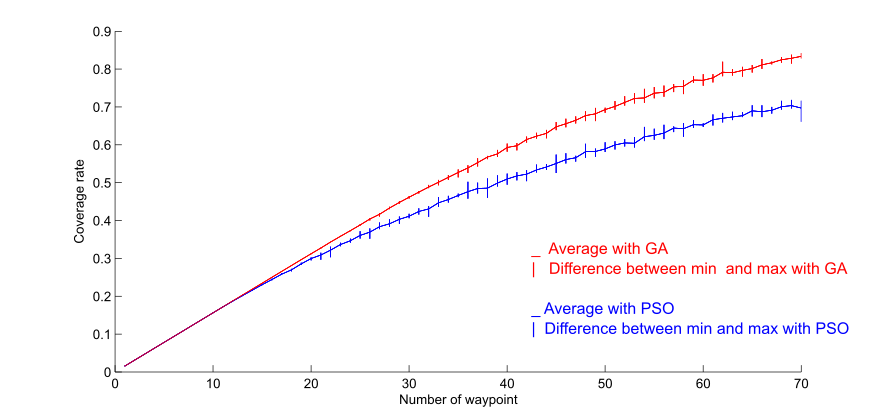
\includegraphics[width=\linewidth]{img/fig8.png}
  \caption{ Comparison of eight solutions given by the GA, with eight solutions given by PSO algorithms with a fixed altitude ($z$ equal to 1) in the big room 240x160. The ground truth for this room equals to 64.}\label{fig:bigRz1}
   \endminipage\hfill
\end{figure}
%
%
\begin{figure}[!]
\minipage{0.99\textwidth}
  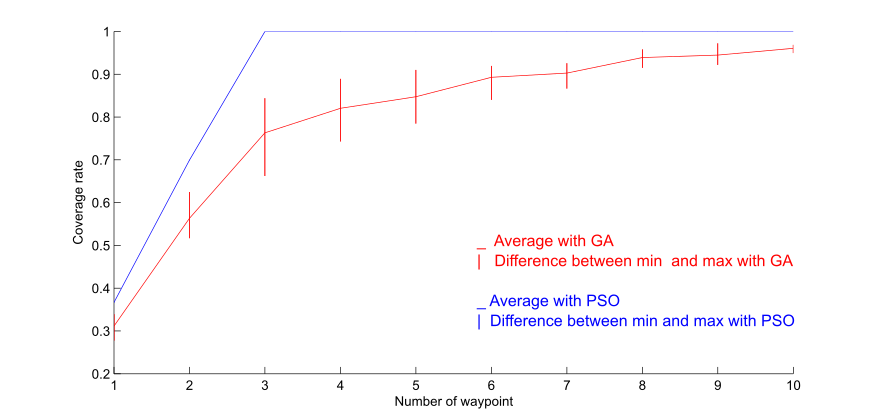
\includegraphics[width=\linewidth]{img/fig9.png}
  \caption{Comparison of eight solutions given by the GA, with eight solutions given by PSO algorithms with a Z between [1/2; 2] in the room with L shape 120x80 and ground truth equal to 15.}\label{fig:RLz2}
   \endminipage\hfill
\end{figure}
After performing the several experiments (see Table \ref{table:table1}), it appears that the GA and PSO algorithms are close in performance in numerous case. Among several experiment of the DoE some particularity appear despite the globally close result of GA and PSO. Also as expected the RS is always the worst solution.
 In the following subsection  just few experiment are taken to illustrate some interesting phenomena specific to the GA and PSO for our problems.

In the case where the search space is large and numerous dimension have to be optimized the GA appear globally more efficient as in Figure \ref{fig:bigRz1}. In contrary in this case (big room with z=1) the PSO give a very bad answer close then simple RS.
%What is appearing in some case as in Figure \ref{fig:bigRz1} is the  GA is much more efficient where the search space is large (big room and big number of cameras),  as the example in Figure \ref{fig:bigRz1}. 
 Instead, PSO is more effective for optimizing small areas as in Figure \ref{fig:RLz2}. In the small room in L shape with a $z$ between 1/2 and 2, the PSO reach quickly (quicker then the 10 000 calls) to the optimal solution. Where here the optimal solution is known and equal to GT. In the same case the GA propose an optimized solution (compared then the RS) but far from the PSO.
 
 This efficiency can be explained by the small variation of the solution introduced by the PSO. However, this small variation is not enough to find an optimized solution in a big search space that occurs when many cameras are required or when the local minimum is deeper. The PSO appear really efficient in a relatively small search space where the number of dimension to optimize is not to high.
 On the other hand the variety  introduced by the GA allows the escape from local minima. This variety is helpfully  in the big search space in order to explore quickly a wide part of it. The variety introduced by the GA became an handicap for a more fine optimization. That explain the bad result obtained during the experiment is a small room. Variety of the GA negatively affect the accuracy of the solution and may require a further optimization step to refine. 
 
%-------- ajouté un exemple entre 2 forme differente qui on un resulta proche 
------------ file Grafig roomShape.txt-----\\
The DoE have been design with different shape in order to see the impact of it on the algorithms. What is appearing during the experiment is the low impact of the shape on the result of the algorithms. The experiment made in the small room (120X80) and the small room in L shape with a z between [1/2; 2](see Figure !!! and Figure !!!). The graphics (see Figure !!! and Figure !!!)  present a similar result, proof of the small impact of the shape on the algorithms.
 This small impact can be explained by the use of meta-heuristic (as PSO and GA) and not by the use of an heuristic  much more dependent of the shape (and the constraint). 
 
Thanks to that we know the two algorithms can be used for a more complex shape as that will be presented in the following experiment.

 





% Following the comparison of the 2 algorithms, the GA seems more suited for finding UAV waypoints especially if it navigates in a large room or  outdoor scenes.
%Furthermore, our comparative study demonstrates that the GA is less dependent on the shape of the area to cover. \\
%------------------
%According to the previous results, the genetic algorithm will be used during future work with no restriction at the convergence point to optimize the positioning of the waypoints in the bigger areas seen in Section  \ref{coverageOutDoor} such as in Figure \ref{subfig:satimg+mask}.\\
%---------------

%fill with the jirs 
%	\subsection{DoF Design of Experiment}
%	\subsection{Result}
%	\subsection{Explication}

\section{Hybrid GA PSO.}
% ref: 76* 77* 
 

% l'hybridration peut permetre de tiré avantage des 2 algo
% \begin{itemize}
%  \item interer de l'hybridation (avantage du PSO sur l'optimisation locale et du GA) 
% \item les forme d'ibridation possible 
% \item la plus aproprier dans notre cas et pourquoi 
% \item les experience ( the experimentation  was done in the Big room in L shape as the \ref{fig:Rooms_shapes}.e)
% \item les resultats
% \end{itemize}
Thanks to the experiment done and presented in the previous section (see \ref{sec:GAvsPSO}) the GA and PSO are two algorithms efficient and complementary to solve the problem of camera positioning in the complex and potentially vast area.
  To summarize the previous comparison, it is difficult to rank the two algorithms in all the environments. GA and PSO have both advantages depending on the area and the number of cameras. GA is better in the big search space and several dimension to optimize. When PSO is efficient to refined faster the solution.
 The hybridization can be the solution to optimize the camera positions in all the condition. The aims of the hybridization is to exploit the better of both algorithms, trying to further refine the solution. 

   77*\cite{c13}.
\subsubsection{The different hybridization.}

In Premalatha al et 76*  propose tree different solution to hybrid the GA and PSO: 
\begin{itemize}
\item  GA and the PSO are used in parallel. The best solution between both algorithms is used into the other algorithm. 
For example: If the best solution at the end of the first generation is from PSO, this solution is used as a new individual for the crossover on the GA. Or if the best solution is from the GA, this good individual is used in PSO as best particle for the next draw. This operation continue until the convergence of both algorithm.   
%(LA MEILLEURE SOLUTION DES DEUX EST INJECTEE DANS L'AUTRE : CA VEUT DIRE QUOI ? ET TEL QUE DECRIT, CE N'EST PAS DU PARALLELE ! MIEUX EXPLIQUER)
 
\item The GA is used to introduce variety on the PSO, when the PSO is stagnating. The stagnated state are reach when no solution upgrades after a predefined number of iteration. In this case the GA introduces variety by proposing an other solution to PSO. This hybridization have to be manage carefully due to this high risk of non convergence. 

\item The GA is used until the convergence point. When the GA converge to a solution, the PSO is used to refine  with one more optimization. This solution is costly in time due to this double optimization and this double convergence. Finally this hybridization uses the GA optimization as an initialization for the PSO.\\
\end{itemize}

The last hybridization using GA as initialization for PSO is probably one of the most suitable for the problems of camera positioning in a large area. 
Based on the previous experiment the  GA operated efficiently  and required to develop a  %good and need to have help for refined 
solution.  %(PHRASE A REVOIR). 
In this case the GA can be a very good initial guess for the PSO. \\

In Shi et al 77*\cite{c13} the hybrid PSO GA was studied for 6 different problems listed F1 to F6. The 6 problem have a global optimal knew.  In this article [77*] the different problems are used to demonstrate the efficiency of hybrid PSO GA and search the appropriate set up for the parameters. One of the interesting aspect presented in [77*] is the importance to find optimized parameters to each algorithms. 
The parameters of the algorithms have to be adapted to the hybridization.
 In our case the GAPSO is used with in a first time a GA and a PSO next to refine the solution. In this case the GA have to introduce even more variety in order to be more efficient. Consequently the GA have to be modified to have a mutation ratio higher.   



\subsubsection{Experimentation.}
To compare the efficiency of the hybridization GAPSO to the GA, one experimentation is proposed.
The experimentation followed the rule fixed during the comparison as in Table \ref{table:table1}. %\\
It appears the big room in L shape as the Figure \ref{fig:Rooms_shapes}.e is the most suitable to test the hybridization.  % (POURQUOI ???).
The L shape room proposes a big search space which can requires a big amount of cameras to cover it. This configuration is the most likely to be improved on different situation, also closer to a realistic configuration.\\
The proposed experiment use the GA for a maximum of 100 generations and the GA solution as a initialization for the PSO. Also the PSO is lock at 100 iterations. %(C'EST L'EXPERIMENTATION QUI PROPOSE ?). \\%Finally the GAPSO are used for an amount around 20000 call of the cost function or the GA use onnly 10000call but the result of GA wiht 20 000 call are similaire then the 10000 (show fig). like that the encreasing is due to the hibridization and not to the morte time computation allowed. 
The set-up of the GA have been slightly change by increasing the mutation ratio and the PSO is also adapted by reduce the inertia. Also a dynamic inertia can be efficient few test was quickly made to test with a mush slower inertia with a small increment  of it at each iteration. This method does not give a significant gain and was preferred to a PSO with a slightly lower inertia parameter (around 0.4).
\begin{figure}[t]
\minipage{0.85\textwidth}
  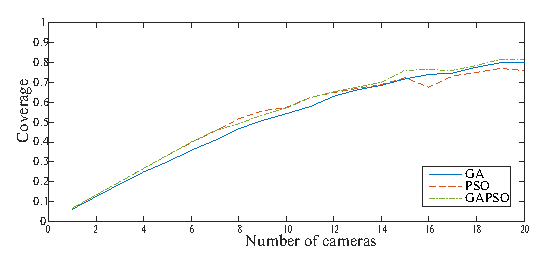
\includegraphics[width=\linewidth]{img/GAPSO_GA_PSO3.eps}
  \caption{comparison between GA PSO and the hybridization of GAPSO.
}\label{fig:GAPSO}
  \endminipage\hfill
\end{figure}

 \subsubsection{Result and comment.}
  
%\begin{figure}[t]
%\minipage{0.95\textwidth}
%  \includegraphics[width=\linewidth]{HibridLroomGAPSO2.png}
%  \caption{GA vs GAPSO.
%}\label{fig:GAPSO}
%  \endminipage\hfill
%\end{figure}

The big room in L shape was used to perform a simple GA and a simple PSO as introduce previously and the GAPSO as explained just before. In the Figure \ref{fig:GAPSO} it is appearing the hybridization of GAPSO increases slightly the percentage of coverage.%(around 0.0002 and 0.107 point of percentage)
This graphic can be split in 2 part, the left side with a relatively low number of cameras to pose (until 15) and the right part with more cameras. To remember in this experiment for each cameras is defined in x y and z that mean for 15 cameras 45 dimensions have to be optimized.
The too side of the graphic show efficiency  of the different algorithms and confirmed  the mechanism of GA and PSO.
The PSO is more efficient in the beginning when the numbers of dimension to optimize is reduced. Otherwise as we saw previously the GA is efficient in the big search space and with a big amount of dimension to optimize the GA is became better than the PSO in the right part of the graphic \ref{fig:GAPSO}. 
The GAPSO propose a solution in the left part of the graphic \ref{fig:GAPSO} equal or a bite better then the PSO. In the right part of the graphic \ref{fig:GAPSO} the GAPSO propose a solution more refine then the simple GA. This refinement is due to the PSO ability to optimize the solution from the first optimization (GA). 

Finally the biggest advantage of the GAPSO is to propose  most of the time the best solution and some time slightly better by combining the advantage of both algorithms. 
The GAPSO can reduce the limitation of the GA and help to go deeper in the optimization process.The GAPSO  beside to upgrade the solution initially proposed by a simple GA or PSO offer more flexibility and allow only one solution to be efficient for the big or small search space despite the number of dimension to optimize.
Despite these great advantage (better solution and more flexibility).
The principal inconvenient of the GAPSO is due to this double convergence. In fact with an hybrid GAPSO as we decide to use a GA have to be executed until a convergence or almost and in the second time optimize with a PSO.  Obviously this implementation increase the time of computation.
 
   
% This refinement is due to the PSO ability to optimize the local solution. As we saw previously the GA is efficient in the big search space and with a big amount of dimension to optimize, but the solution gives the GA need some local adjustment to be better. The GA has few limitation to go deeper in the optimization process but this weakness is partially corrected by the hybridization. The principal advantage hybridization is the ability to keep the benefit of both algorithms. The Figure \ref{fig:GAPSO} show that the GAPSO proposes most of the time the best solution or equal to the best solution by combining the advantage of both algorithms. 
%	\subsection{memetic ???}
%		\subsubsection{DoF}
%		\subsubsection{Result}
%		\subsubsection{Conclusion}
		
\section{Experiment}
	\subsection{No obstacle }
	\subsection{Rectangle obstacle}
	\subsubsection{With mask}
	\subsection{For big area}
		\subsubsection{map 1}
		\subsubsection{map2 torcy}
		\subsubsection{map3 calvisson}
		


%%%%%%%%%%%%%%%%%%%%%%%%%%%%%%%%%%%%%%%%%%%%%%%%%%%%

 


